% \subsubsection{Application Demos} We present extensive results of avatar animations to show the capability and potential of bringing avatar animation empowered by {\nameofmethod} to next level. We show that {\nameofmethod} serves as a strong foundation model for audio-driven avatar animation, which can synthesize vivid and high-fidelity videos. As shown in Fig. \ref{fig:application-audio}, the generated videos display life-like facial expressions with synchronized lip motions. It also synthesizes videos with rich background dynamics. We also show that {\nameofmethod} boosts the performance of pose-driven animation largely in many aspects, including ability of following complex poses, maintaining details of garment texture and ID consistency along frames (Fig. \ref{fig:application-pose-compare}). In addition, tunning {\nameofmethod} to animate characters shows remarkable ability of generalization. As shown in Fig. \ref{fig:application-pose}, we can animate not only realistic characters, but also non-realistic ones, surprisingly including but not limited to cartoon figures, pottery figurines, anthropomorphic animals, and many others. Fig. \ref{fig:application-expr} shows that finetuning \nameofmethod with added adapter layers synthesize vivid portrait expression videos. It is able to mimic facial motions such as eye gaze, lip motion accurately while maintaining high ID consistency. Lastly, we show that hybrid condition control reveals the potential of fully controllable and editable avatars. As shown in Fig. \ref{fig:application-pose-expr}, we can animate a static avatar character with driving templates from different sources. This hybrid control paradigm paves the route from demo to applications for avatar animation. In addition, we show that hybrid controllability generalizes to both realistic and non-realistic characters (Fig. \ref{fig:application-pose-expr-2}).

% \begin{figure}
%     \centering
%     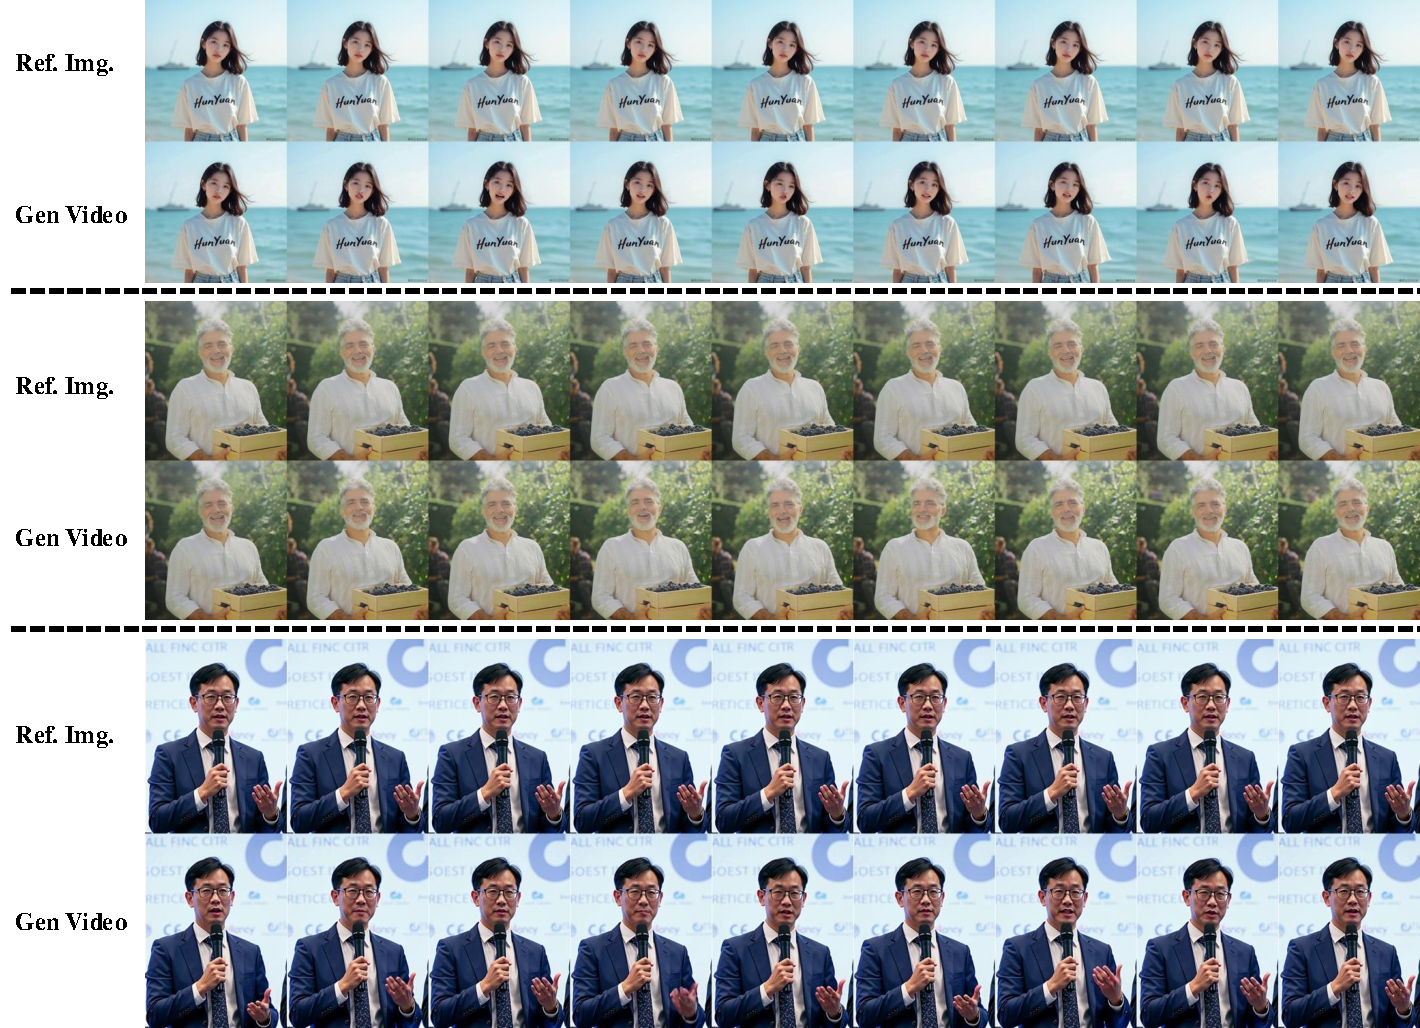
\includegraphics[width=\linewidth]{applications/app_figures/audio-1.pdf}
%     \caption{\textbf{Audio-Driven}. {\nameofmethod} can generate vivid talking avatar videos.}
%     \label{fig:application-audio}
% \end{figure}

% \begin{figure}
%     \centering
%     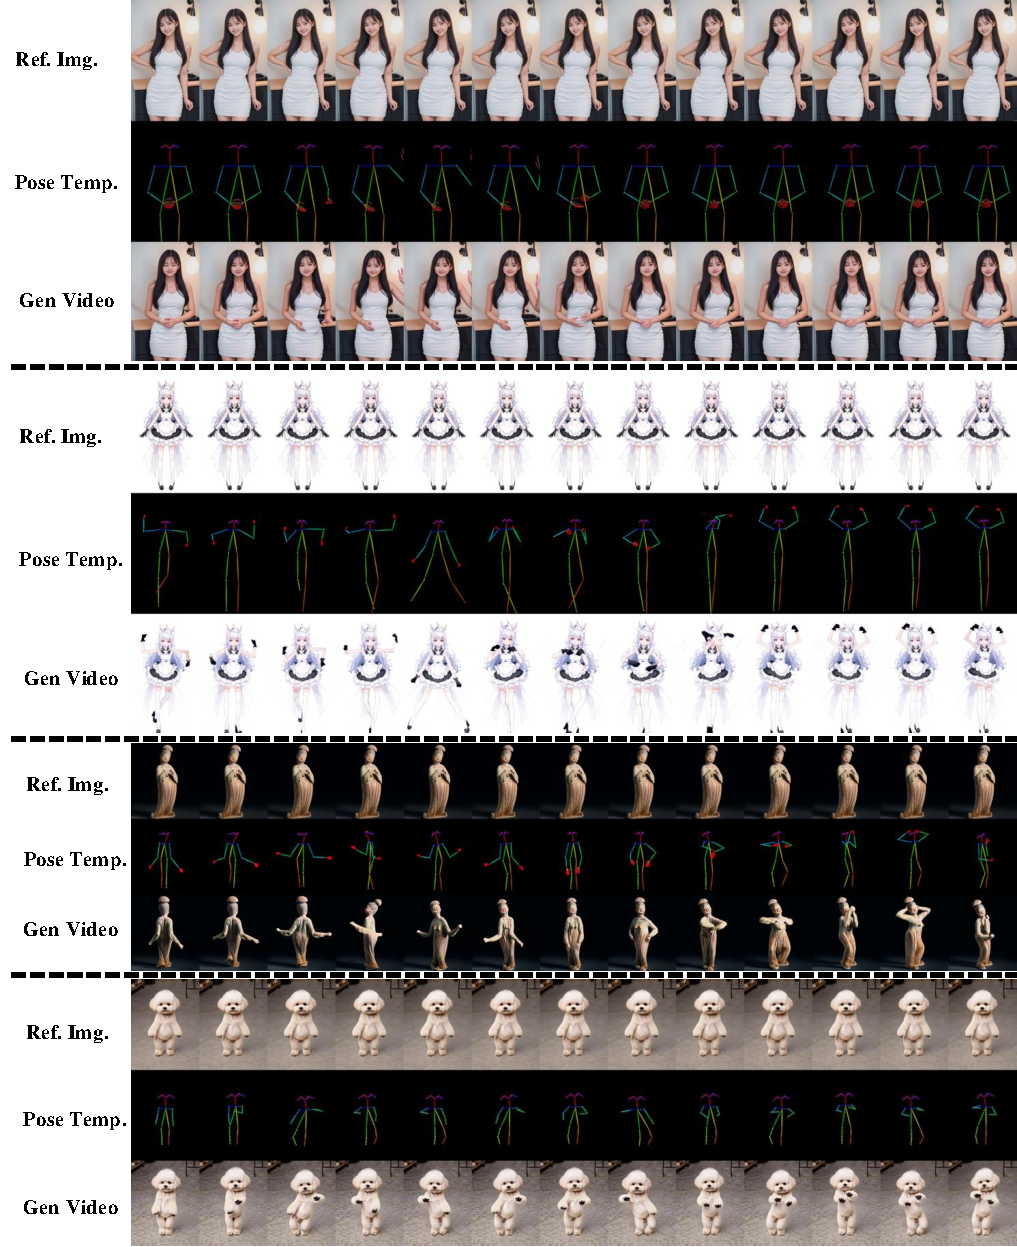
\includegraphics[width=\linewidth]{applications/app_figures/pose.pdf}
%     \caption{\textbf{Pose-Driven}. {\nameofmethod} can animate wide variety of characters with high quality, ID consistency under various poses.}
%     \label{fig:application-pose}
% \end{figure}


% \begin{figure}
%     \centering
%     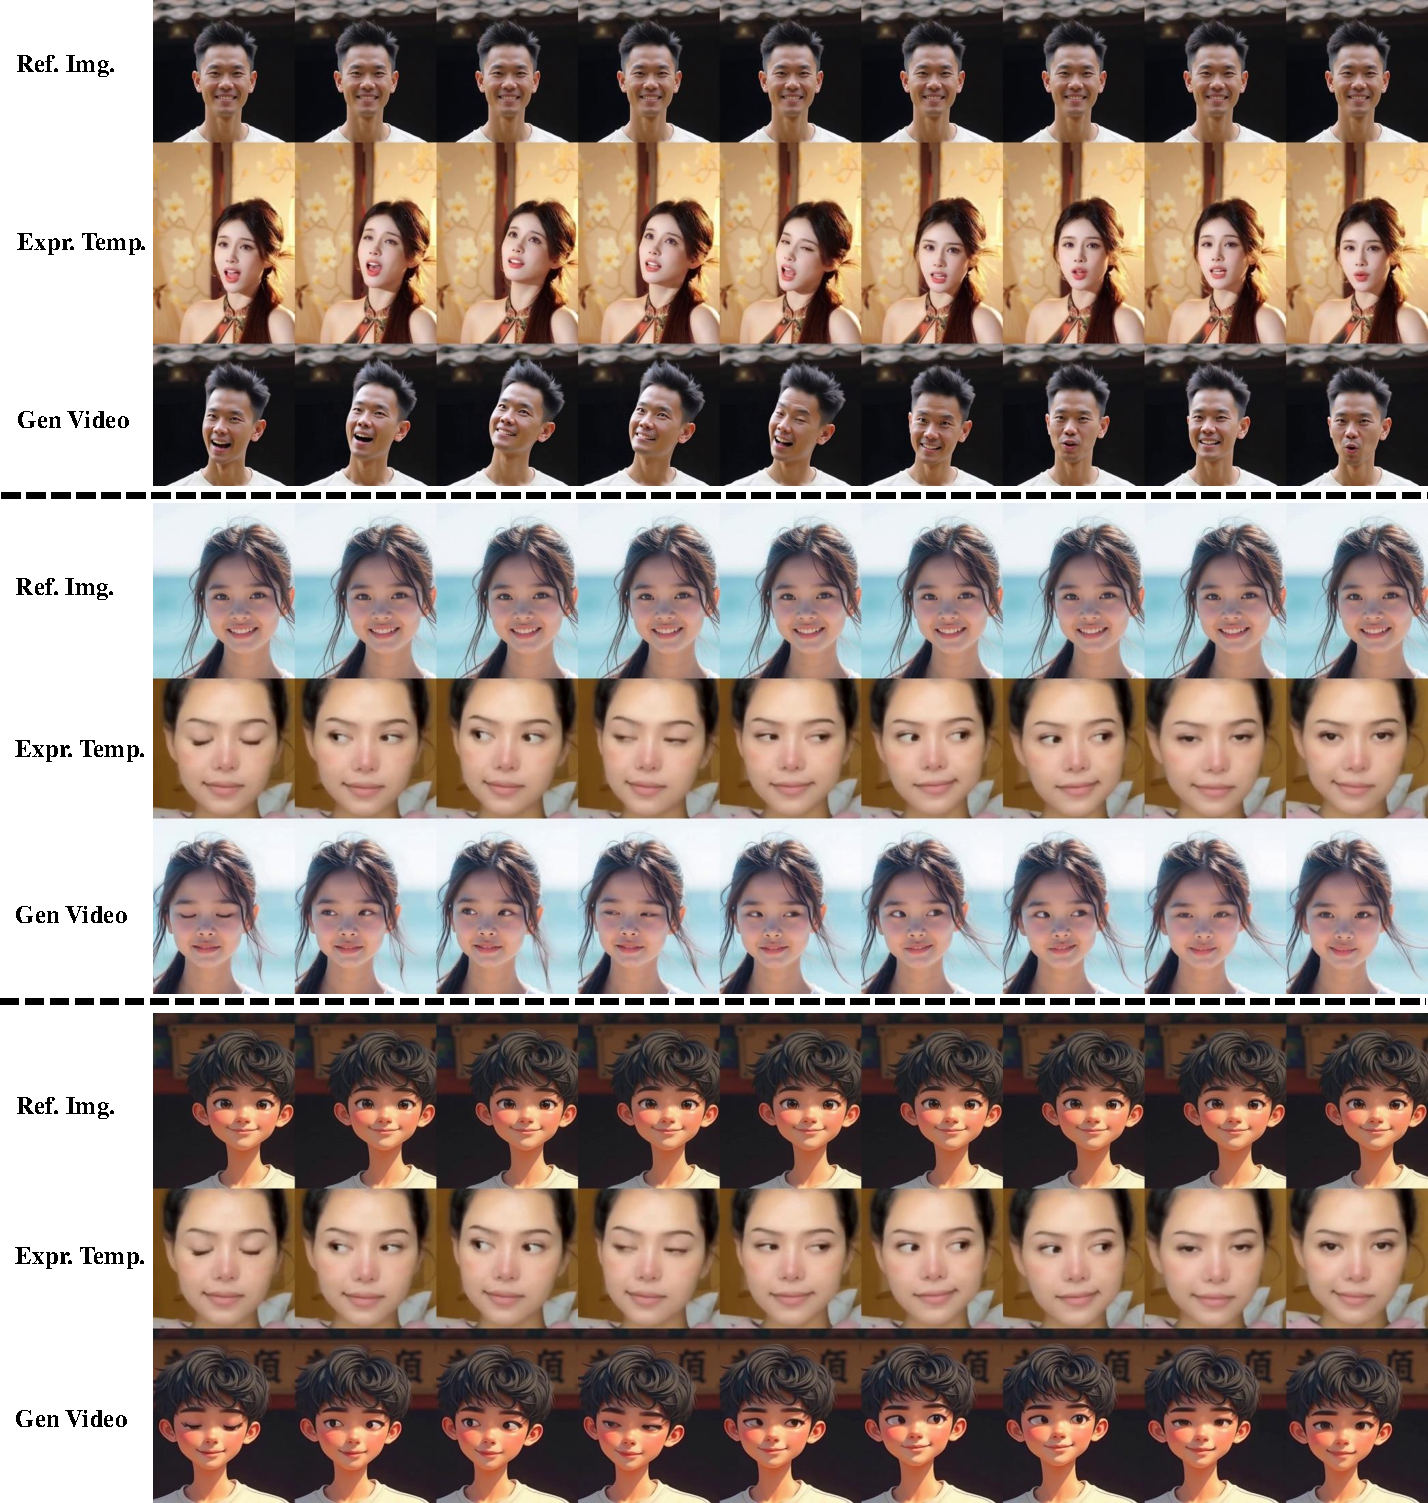
\includegraphics[width=\linewidth]{applications/app_figures/expr-1.pdf}
%     \caption{\textbf{Expression-Driven}. Our method can animate facial expressions of wide-variety of avatar styles.}
%     \label{fig:application-expr}
% \end{figure}

% \begin{figure}[h]
%     \centering
%     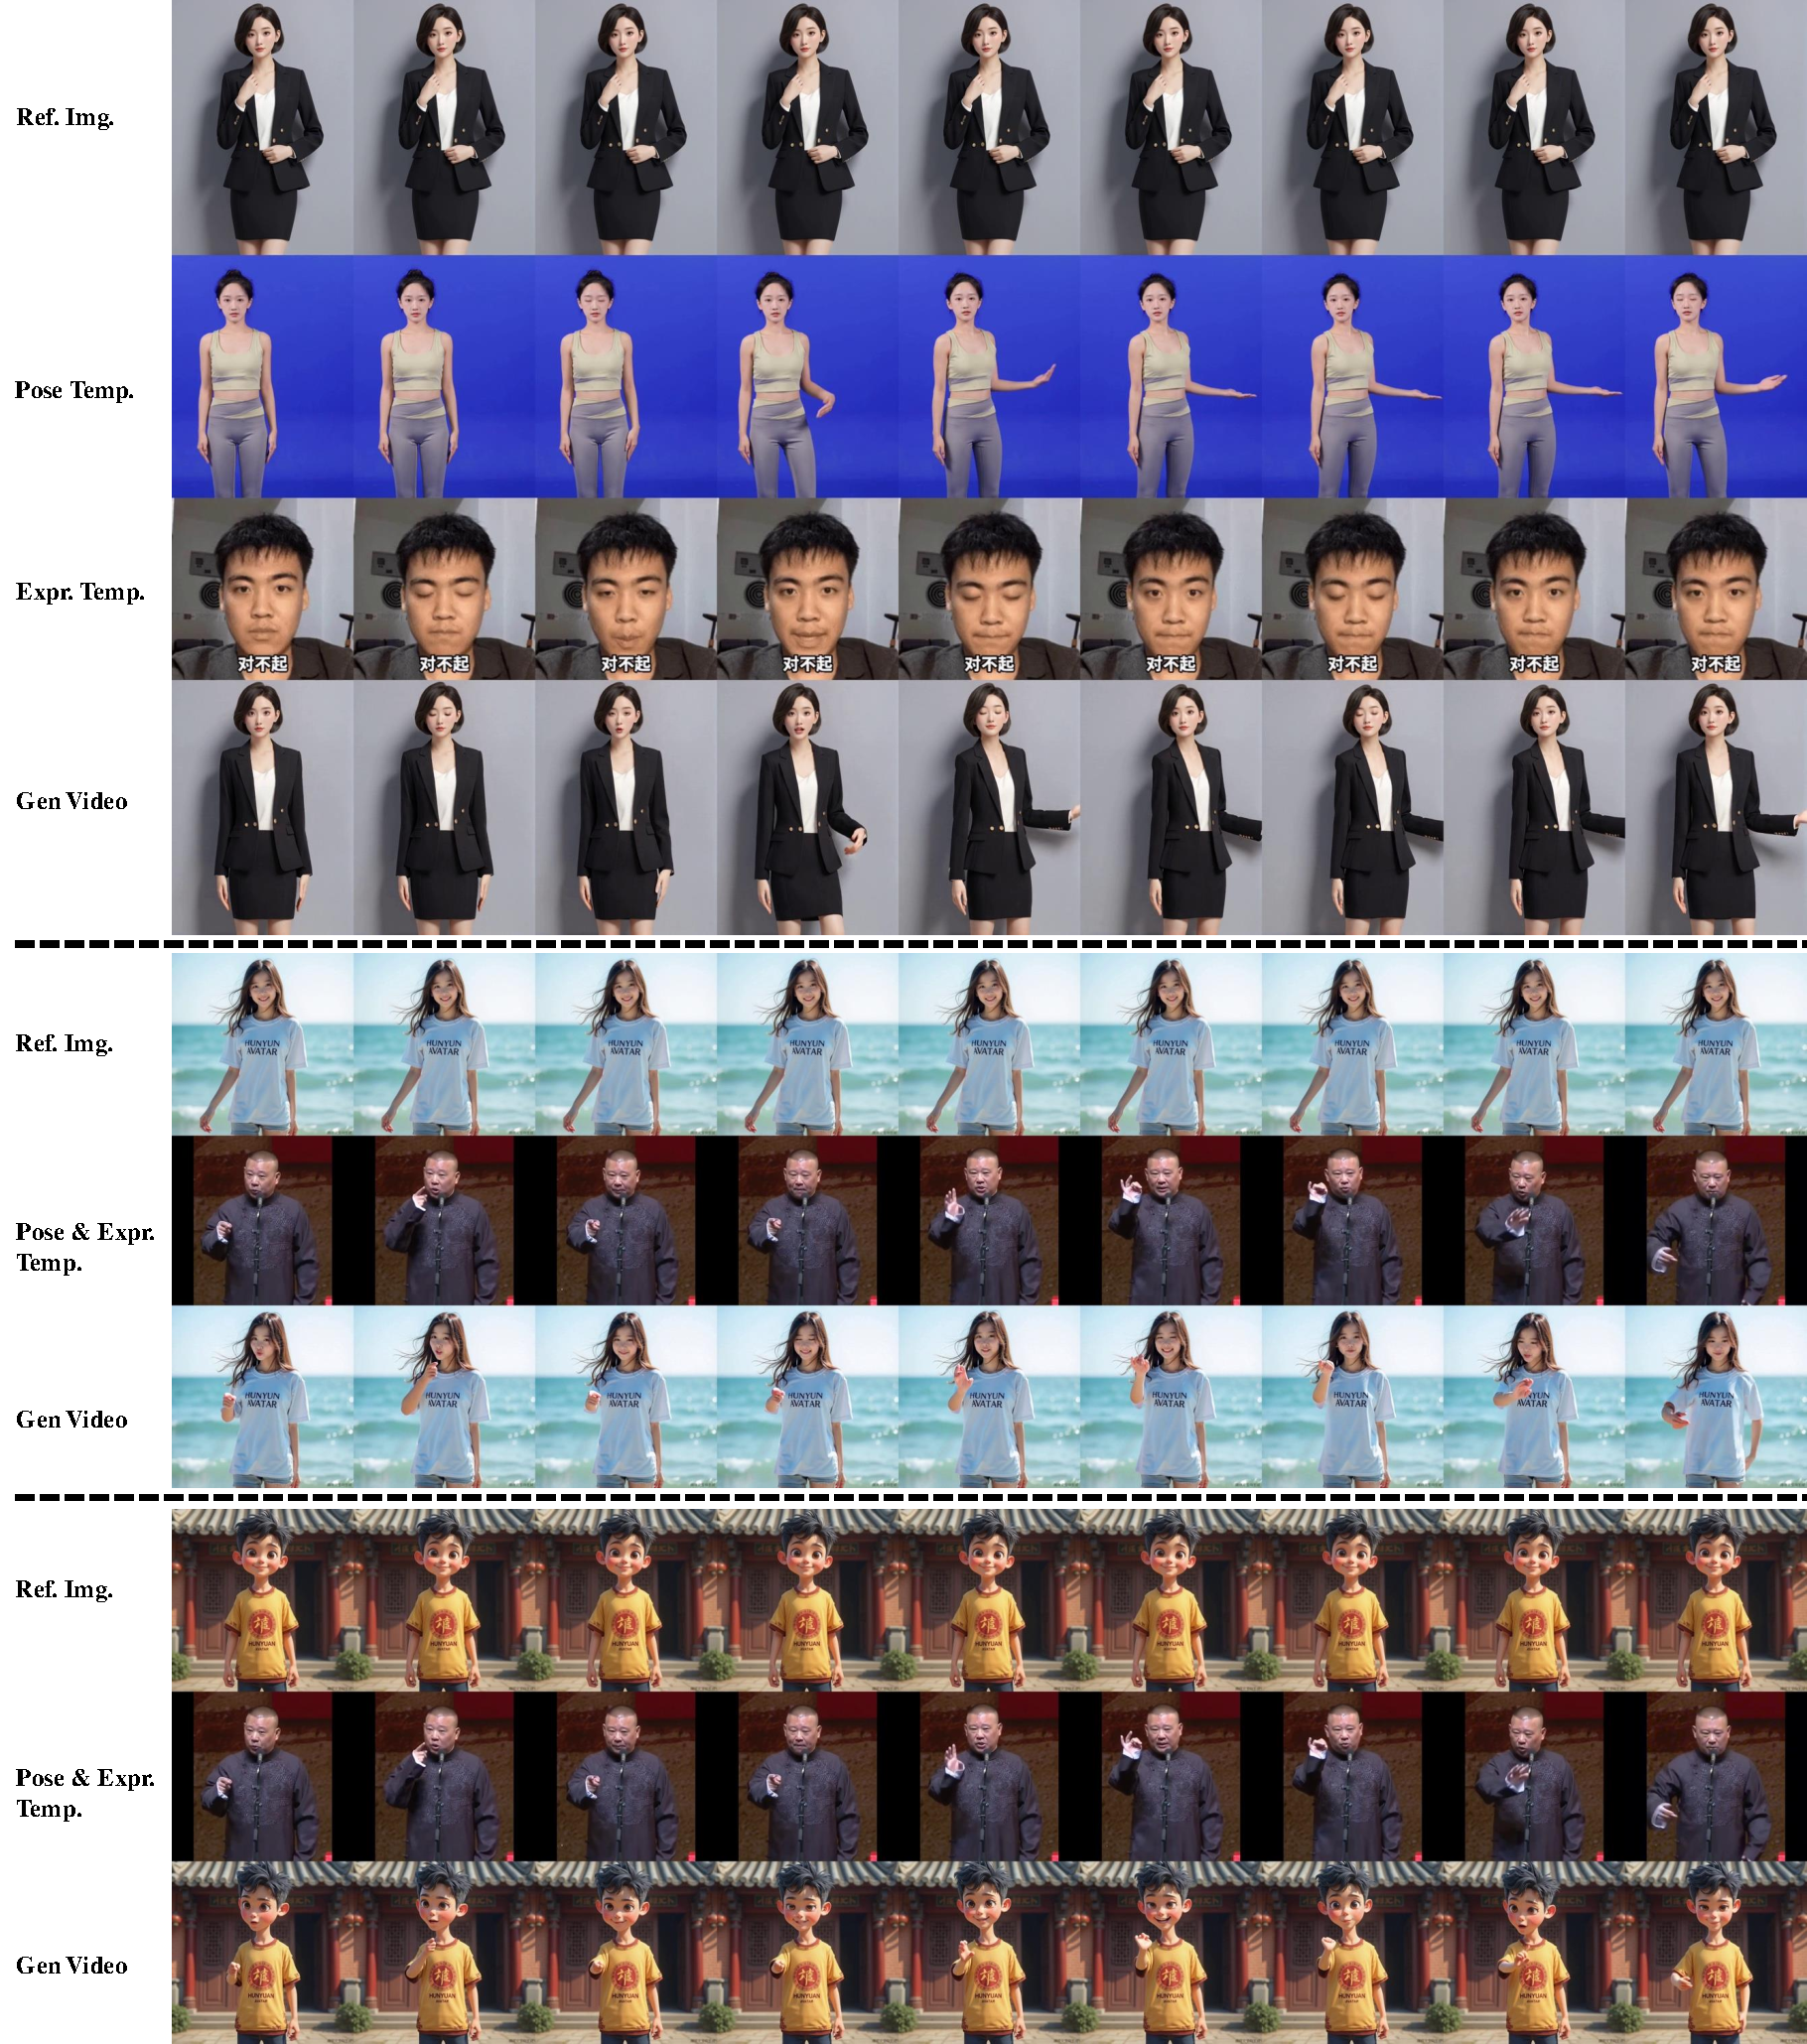
\includegraphics[width=\linewidth]{applications/app_figures/pose-expr-1.pdf}
%     \caption{\textbf{Hybrid Condition-Driven}. Our method supports full control with multiple driving sources across various avatar characters.}
%     \label{fig:application-pose-expr}
% \end{figure}

\subsection{Application Demos} We present extensive results of avatar animations to show the superiority and potential of bringing avatar animation empowered by {\nameofmethod} to next generation.

\paragraph{Audio-Driven}Fig. \ref{fig:application-audio} shows that {\nameofmethod} serves as a strong foundation model for audio-driven avatar animation, which can synthesize vivid and high-fidelity videos. We summarize the superiority of our method in three folds:

\begin{itemize}
    \item \textbf{Upper-body Animation.} Our method can drive not only portrait characters, but also upper-body avatar images, enlarging its range of application scenarios. 
    \item \textbf{Dynamic Scene Modelling.} Our method can generate videos with vivid and realistic background motion, such as the wave undulation, crowd movement, and breeze stirring leaves. 
    \item \textbf{Vivid Avatar Movements.} Our method is able to animate the character talking while gesturing vividly with audio solely.
\end{itemize}

\paragraph{Pose-Driven}We also show that {\nameofmethod} boosts the performance of pose-driven animation largely in many aspects in Fig. \ref{fig:application-pose}:

\begin{itemize}
    \item \textbf{High ID-Consistency.} Our method maintains the ID-consistency well over the frames even with large poses, making it face-swapping free, thereby, could be used as real end-to-end animation solution.
    \item \textbf{Following Complex Poses Accurately.} Our method is able to handle very complex poses such as turning around and hands crossed.
    \item \textbf{High Motion Quality.} Our method has remarkable capability in dynamic modelling. For instance, the results show promising performance in terms of garment dynamics and texture consistency.
    \item \textbf{Generalizability.} Our method presents surprisingly high generalizability. It can animate wide variety of avatar images, such as real human, anime, pottery figurine, and even animals. 
\end{itemize}

\paragraph{Expression-Driven}Fig. \ref{fig:application-expr} presents how {\nameofmethod} enhances the portrait expression animating in three folds:

\begin{itemize}
    \item \textbf{Exaggerated Expression.} Our method is able to animate given portrait to mimic any facial movements even with large poses and exaggerated expressions.
    \item \textbf{Mimicing Eye Gaze Accurately.} We can control the portraits' eye movements acurately given any expression template, even with extreme and large eye balls movements.
    \item \textbf{Generalizability.} Our method has high generalizability. It can animate not only real human portraits, but also anime or CGI characters.
\end{itemize}

\paragraph{Hybrid-Driven} Lastly, we show that hybrid condition control reveals the potential of fully controllable and editable avatars in Fig. \ref{fig:application-pose-expr}. We highlight the superiority as follow:

\begin{itemize}
    \item \textbf{Hybrid Condition Control.} For the first time, our method is able to conduct full control over body and facial motions with siloed or multiple signals, paving the route from demo to applications for avatar animation.
    \item \textbf{Half-body Animation.} Our method supports upper-body full control, enabling rich editability while maintaining high quality and fidelity.
    \item \textbf{Generalizability.} Our method generalize to both real human images and CGI characters. 
\end{itemize}


% \begin{figure}
%     \centering
%     \includegraphics[width=\linewidth]{applications/app_figures/pose-compare.pdf}
%     \caption{\textbf{{\nameofmethod} Boosts Pose-Driven Animation in Many Aspects}. (a) It maintains garment details (sleeves). (b) Better pose following (fingers). (c) Higher ID consistency (faces).}
%     \label{fig:application-pose-compare}
% \end{figure}

% \begin{figure}
%     \centering
%     \includegraphics[width=\linewidth]{applications/app_figures/pose-expr-5.pdf}
%     \caption{\textbf{Animating Wide-Variety of Avatars}. Our method can animate both realistic character (upper pannel) and cartoon style (lower pannel).}
%     \label{fig:application-pose-expr-2}
% \end{figure}